\section{Data}

\subsection{Light Bulbs and the Solar spectrum}
For this part, we plotted the meassured intensity of the light as a function of 
wavelengths, and determined at which index of wavelength, the peak of highest
intensity was at. This wavelength corresponds to a temperature as described in
\cref{eq:wien} to calculate the temperature $T$.
For the three meassurements of the solar spectrum, we took an average. All the
temperatures are shown in \cref{tab:temp}.
\begin{table}[h]
\centering
\begin{tabular}[h]{lr}
\toprule
Source & Temperature\\
\midrule
Halogen       & $\SI{4736}{\kelvin}$\\
Diode         & $\SI{4842}{\kelvin}$\\
Energy-saving & $\SI{4829}{\kelvin}$\\
Solar average & $\SI{5663}{\kelvin}$\\
\bottomrule
\end{tabular}
\caption{Surface temperatures of the given sources, as determined by wiens
displacement law.}
\label{tab:temp}
\end{table}
Our meassurements of the three lamps are shown compared to the three solar
spectra on \cref{diode}, \cref{halogen} and \cref{Energy-saving}.

\begin{figure}[h!]
\centering
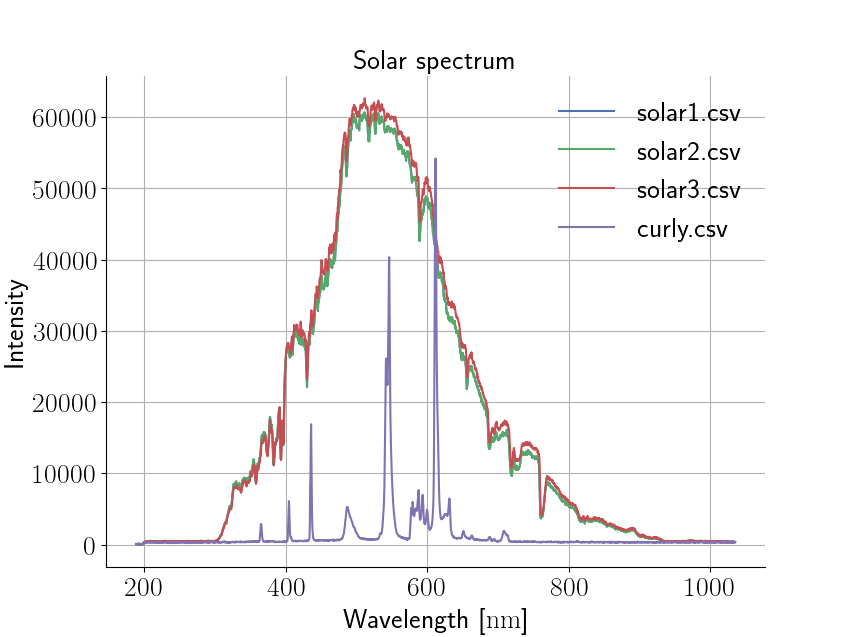
\includegraphics[width=0.65\textwidth]{SolarComparison0}
\caption{The spectrum of the diode-based lamp compared to the three meassured spectra of
the sun.} 
\label{diode}
\end{figure}

\begin{figure}[h!]
\centering
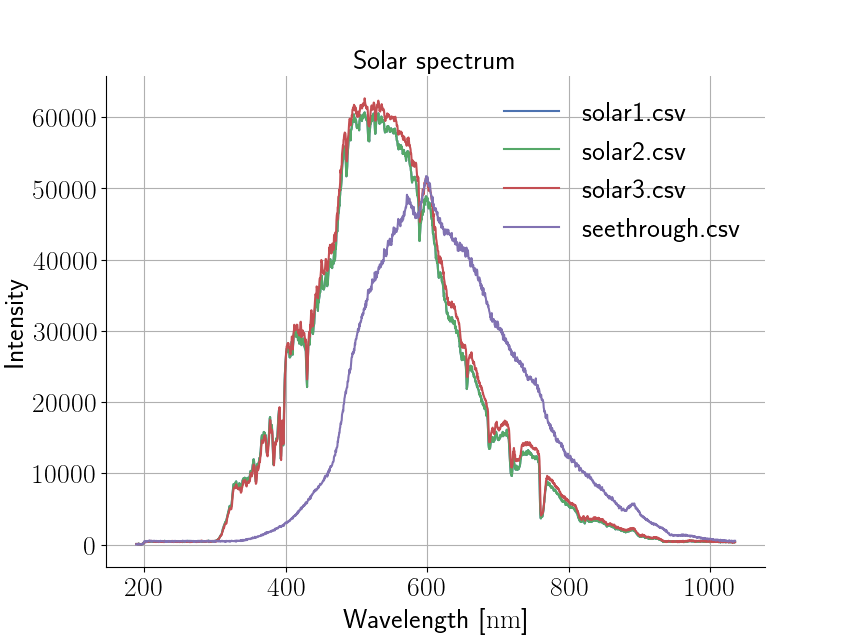
\includegraphics[width=0.65\textwidth]{SolarComparison1}
\caption{Halogen}
\label{halogen}
\end{figure}

\begin{figure}[h!]
\centering
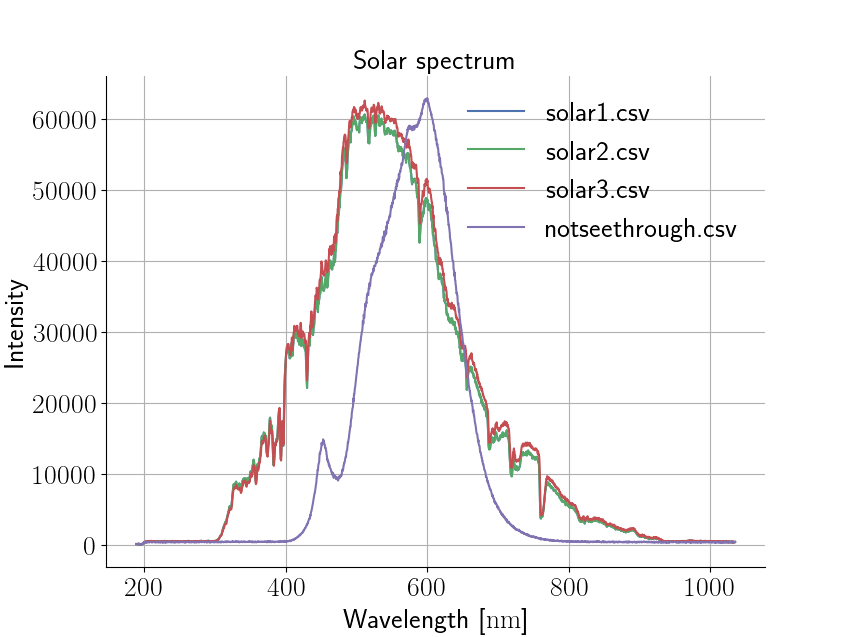
\includegraphics[width=0.65\textwidth]{SolarComparison2}
\caption{Energy-saving lamp}
\label{Energy-saving}
\end{figure}

\subsubsection{Comparison}
The question is, which of our three lamps best represtent the solar spectrum.
From the three figures \cref{diode}, \cref{halogen} and \cref{Energy-saving},
it can be seen, that:

\paragraph{diode}
This spectrum is discrete. Some of the wavelengths are similar to that of the
solar, but it is certainly not a blackbody.

\paragraph{halogen}
This spectrum has its peak displaced further into the yellow color, whereas the
sun has a greenish peak. Nonetheless, it is certainly a better approximation
than that of the diode.

\paragraph{energy-saving}
This spectrum has its peak nearest that of the solar spectrum, and thus shares
the same color. Though it has a smaller full-width-half-maxima than that of the
halogen lamp.

\subsection{Fraunhofer lines}
\begin{figure}[h]
\centering
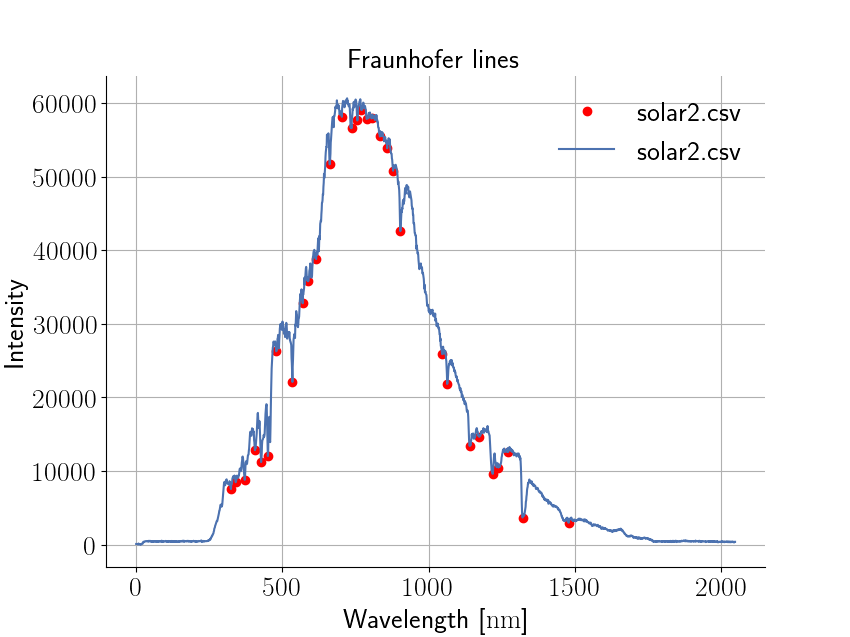
\includegraphics[width=0.65\textwidth]{Fraunhofer}
\caption{The Solar spectra with the local extrema points used for
classification of the Fraunhofer lines}
\label{frauenhofer}
\end{figure}

Comparing the found extremas with the Fraunhofer lines, we have meassured the
following

\subsection{DEL 2: ENERGY TABEL.. AK}

\subsection{Absorption Spectroscopy}
\begin{figure}[h]
\centering
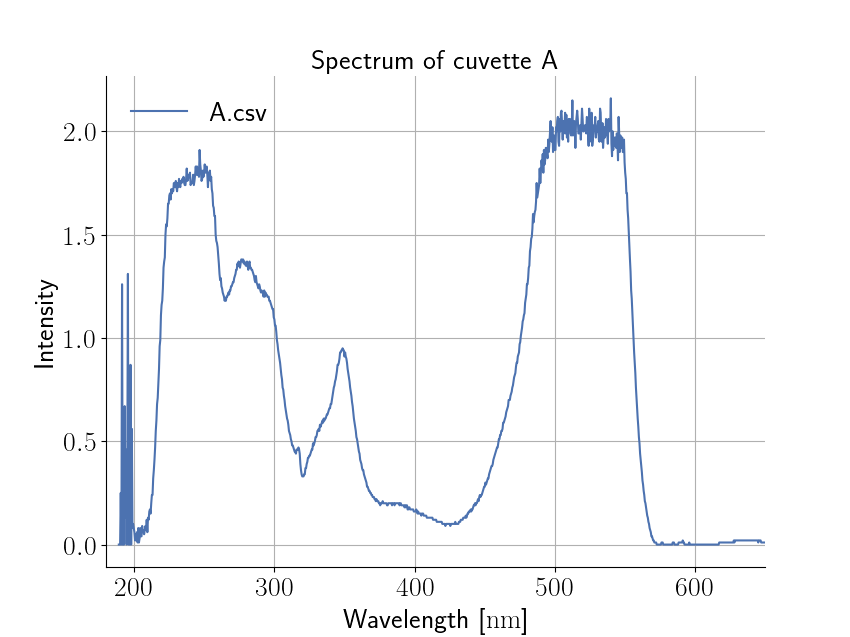
\includegraphics[width=0.65\textwidth]{absA}
\caption{Spectrum of cuvette A: This might just be Rhodamine 6G}
\label{fig:absA}
\end{figure}
\begin{figure}[h]
\centering
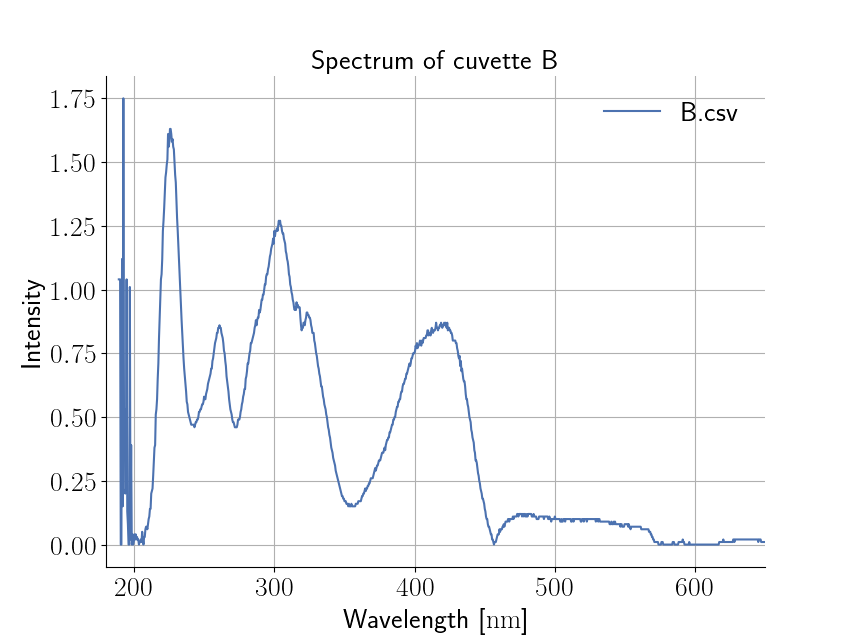
\includegraphics[width=0.65\textwidth]{absB}
\caption{Spectrum of cuvette B. As this seems different from all spectra of
figure 13 (in lab guide), this might just be Kaliumhexacyanoferrat (III)}
\label{fig:absB}
\end{figure}
\begin{figure}[h]
\centering
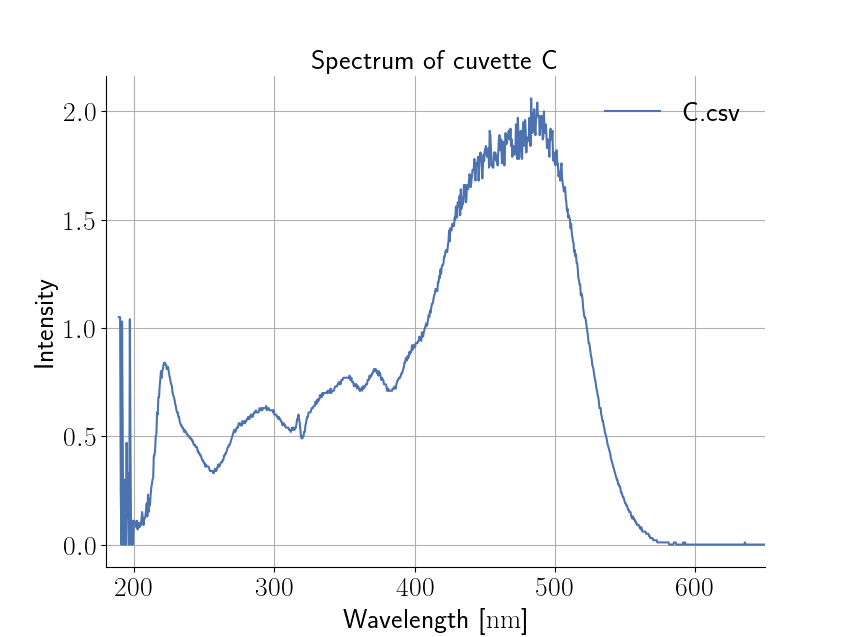
\includegraphics[width=0.65\textwidth]{absC}
\caption{Spectrum of cuvette C. This might just be DCM}
\label{fig:absC}
\end{figure}
